% This file contains the content for the Introduction
\unnumberedformat	    % Change formatting to that of "Introduction" section
\chapter{Introduction} 	% Do not modify section title
%% Modify below this line %%
    
\section{What an IDT does}
In the Academy Color Encoding System (ACES), the Input Device Transform (IDT) converts non-color-rendered RGB image values from a given camera system or other image capture device to ACES RGB relative exposure values.

\subsection{Required behaviors}
The image data produced by the IDT shall

\begin{itemize}
    \item	In the case of D60 illumination, approximate the ACES RGB relative exposure values that would be produced by the RICD\footnote{The spectral sensitivities of the RICD are defined in Annex C of SMPTE ST 2065-1:2008.},
    \item	Approximate radiometrically linear representations of light reaching the focal plane,
    \item	Contain a nonzero amount of flare as specified in the ACES document,
    \item	Use equal RGB relative exposure values to represent colors that are neutral under the illumination source for which the IDT is designed, and
    \item	Approximate a colorimetric response to the scene for the illumination source for which the IDT is designed, though the native camera system response itself may not be colorimetric.
\end{itemize}

\subsection{Optional behaviors}
In addition to the required IDT behaviors, several other behaviors, while not implied by the ACES document, are common enough to deserve mention. At the IDT manufacturer’s discretion, the image data produced by the IDT may

\begin{itemize}
    \item	Be modified in such a way as to minimize artifacts resulting from camera system clipping, including white balance-specific highlight clipping and recovery.
    \item	Be compensated for differences between the chromaticity of neutrals from the white-balanced camera system and the chromaticity of neutrals in the ACES encoding.
\end{itemize}

\subsection{Recommended illumination source support}
The set of IDTs for a given camera system should include IDTs optimized for daylight (CIE Illuminant D55) and tungsten (ISO 7589 Studio Tungsten).

\subsection{Optional illumination source support}
The set of IDTs may include IDTs for common illumination sources such as Hydrargyrum Medium-arc Iodide (HMI) and KinoFlo\textsuperscript{\textregistered{}} lamps.

\subsection{Expectations of IDT input}
An IDT is expected to be applied after the following types of initial processing: dark frame subtraction, noise reduction, flat fielding, demosaicing, conversion to a device-specific RGB color space, and/or deblurring. If, for a particular camera system, linearization or white balance takes place prior to one of the abovementioned processes, then that linearization or white balance shall be excluded from the IDT.

\subsection{Camera system `look; consequences of the IDT}
There is no camera-system-independent `cookbook' procedure for producing optimal IDTs. Camera system manufacturers may differ on how to distribute color analysis error across the set of all possible input colors, and may have different philosophies on neutral chromaticity difference compensation.

Moreover there are an infinite number of possible illumination conditions under which a scene might be captured; even if a manufacturer decided on particular strategies to ameliorate color analysis error and to compensate for the scene neutral chromaticity differing from ACES' neutral chromaticity, `optimal' capture might require an infinity of IDTs.

To avoid confusion and other problems, the Academy recommends this infinity be reduced to the smallest possible number consistent with best cinematographic practice.

As implied by the `Recommended illumination source support' section above, this number could be as low as two (a daylight IDT and a tungsten IDT, paralleling film workflows). Some camera systems may also provide finer-grain control of correlated color temperature (interpolating CCT between daylight and tungsten illumination sources, for example), or may handle `outlier' sources such as HMI or KinoFlo\textsuperscript{\textregistered{}}. The key point of the Academy recommendation is that there be a single differentiating factor between the IDTs offered for a particular digital camera system: the IDT's assumed illumination source.

\subsection{Evaluating IDT output}
An IDT produces image data that have not been color rendered, and that closely maintain the radiometric relationship of the objects in the captured scene as they existed at the camera focal plane. Image data in this state are well suited for inter–facility image exchange, for some sophisticated image operations (e.g. partial or full recovery of highlight detail), for photo-realistic compositing, and for merger with Computer Generated Imagery (CGI) elements.

For critical color evaluation, such image data should be color rendered using the ACES Reference Rendering Transform (RRT), processed by an ACES Output Device Transform (ODT) and viewed using the device and viewing environment specified by the ODT creator. 

\subsection{Relationship of IDT and Look Modification Transform (LMT)}
When a creative choice is made to move the `look' of the captured imagery away from maximum fidelity to the image existing at the focal plane, this change should be effected not by changing the behavior of the IDT, but by post-processing the IDT output with a Look Modification Transform (LMT) or a set of LMTs.

The on-set relationship of the IDT, any LMT or set of LMTs, the RRT and the ODT for an on-set preview device is shown in \autoref{fig:onset}\footnote{ACES and the Digital Cinema Distribution Master (DCDM) encoding are intended for use as image storage encodings. Although it is possible to use the Output Color Encoding Specification (OCES) encoding for image storage, it is primarily a conceptual encoding, a common `jumping-off point' for Output Device Transforms (ODTs), and is thus shown in \autoref{fig:onset} in light rather than in dark gray.}.

\begin{figure}[htbp]
\begin{center}
    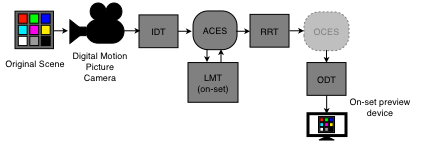
\includegraphics[width=4in]{onset.png}
\caption{}
\label{fig:onset}
\end{center}
\end{figure}

Camera system image data are processed by the IDT prior to the application of any LMT or set of LMTs. This means that whether that LMT or set of LMTs is expressed as a Color Transform Language (CTL) program, or as an American Society of Cinematographers Color Decision List (ASC CDL), a 3D LUT provided by the camera vendor, or some combination thereof, the `look' is being imposed on ACES data.

The LMT or set of LMTs thereafter accompanies the ACES data through postproduction; critical color judgments are made through the concatenation of the `look' that was established on-set and any additional `look' applied in post-production, as shown in \autoref{fig:lmt}.

\begin{figure}[htbp]
\begin{center}
    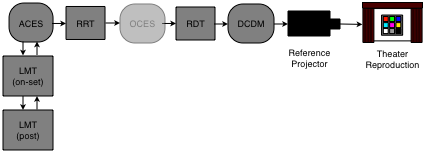
\includegraphics[width=4in]{lmt.png}
\caption{}
\label{fig:lmt}
\end{center}
\end{figure}

Throughout production and postproduction, the `look' established by the cinematographer is carried in parallel with the unmodified ACES data produced by the camera system IDT.

This separation of `look' and unmodified ACES data supports workflows in which the ACES data's approximation of truly accurate colorimetric capture can greatly aid production, such as when the content will be merged with CGI accurately modeling the physical properties of lights and reflectances in the real or virtual scene. It also separates the tasks of capture and of modeling downstream processes such as the transformation of image data to simulate film-based capture.

Finally, the LMT provides a well-defined point where camera manufacturers can provide emulation of traditional camera system controls, allowing the cinematographer to `paint with the camera.'

\section{How an IDT works}
\subsection{Structure of an IDT}
As detailed above, the required and most common optional responsibilities of an IDT are six-fold: linearization, white balancing, clipping, color analysis, neutral chromaticity difference compensation and encoding as ACES RGB relative exposure values. The first typically requires per-channel functions or 1-dimensional lookup tables (LUTs). The second of these is accomplished by per-channel scaling to the RGB data. The third (clipping) can be done simply or in complex manners that attempt to reconstruct or extrapolate clipped values. The fourth and fifth are accomplished together by the application of a 3x3 signal processing matrix and the sixth is a simple uniform scaling of the matrixed RGB channel data. The final resulting image data are ACES RGB relative exposure values.

This document provides a recommended procedure for the creation of an IDT whose core is a 3x3 matrix that converts normalized white-balanced radiometrically linear RGB code values representing a digital camera system's capture of a scene to ACES RGB relative exposure values. In doing so, it fulfills the required functions of an IDT and implements several of the optional behaviors (notably clipping and neutral chromaticity difference compensation.) Building the IDT around a single 3x3 matrix has several advantages:

\begin{itemize}
    \item	It follows standard industry practice\footnote{SMPTE RP 177:1993 (R2003), Derivation of Basic Television Colour Equations}.
    \item  	It allows preservation of neutral camera system RGB code values to be enforced mathematically, and chromaticity is invariant with exposure changes.
    \item	It limits the degrees of freedom of the transform, preventing the transform from following the training set colors too closely at the expense of other colors.
    \item	It introduces a smaller amount of color analysis error in its output than would be the case if RICD emulation and neutral chromaticity compensation were separate, individually-optimized transforms.
    \item	It is readily invertible, allowing for reconstruction of white-balanced radiometrically linear camera system RGB code values from ACES RGB relative exposure values. 
    \item	Its application is simple to understand.
\end{itemize}

\subsection{Linearization}
Linearization is constrained to occur between initial acquisition of sensor data and white balance. It is interspersed with operations such as dark current subtraction, pixel defect correction, flat-fielding, and in some cases demosaicing and deblurring. In some camera systems, it may be necessary to incorporate linearization into the IDT; in other camera systems, linearization may be performed prior to the application of the IDT as part of performing those other operations. The result of linearization is an RGB encoding in which RGB channel values are directly and linearly proportional to radiometric energy at the camera focal plane.

\subsection{White balancing}
The linearized RGB image data are scaled by RGB channel multipliers such that a perfect reflecting diffuser in the scene, illuminated by the scene adopted white, would be encoded with equal RGB channel values.

Although the channel multipliers could conceivably be specified explicitly and independently, it is anticipated that many camera systems will set the channel multipliers providing the white balance when the cinematographer chooses an IDT. The absolute values of the channel multipliers are such that white-balanced linearized RGB image data representing a captured perfect reflecting diffuser illuminated by the scene adopted white would have equal RGB channel values all being unity.

White balance is constrained to occur after linearization and before clipping. In systems where white balancing must precede operations which cannot be done inside the IDT (demosaicing, for example) white balance will need to be done external to and prior to application of the IDT.

\subsection{Clipping}
The linearized, white-balanced RGB image data are clipped prior to matrix application. This recommended procedure imposes a simple clipping method by which all RGB channel values are clipped to the maximum RGB values imposed or implied by the original camera system encoding.

More ambitious clipping strategies are possible but as these are typically proprietary, and may depend on information being available in a device-dependent way (they may, for example, rely on the ability to examine the values of neighboring pixels), such clipping strategies are not discussed in this document.

\subsection{Matrix application}
The linearized, white-balanced clipped RGB image data are multiplied by a 3x3 matrix. This matrix implements two functions simultaneously: color analysis, and neutral chromaticity difference compensation.

Color analysis attempts to minimize differences between the spectral responsivities of actual camera sensors and the spectral responsivities of the RICD, a hypothetical colorimetric camera whose spectral sensitivities are exactly expressed as linear transformations of the CIE 1931 colorimetric observer. Such differences can be minimized but not entirely eliminated. The distribution of residual error is an expression of the manufacturer's prioritization of some colors over others, in particular, of `memory' colors over colors rarely found in digital motion picture production.

Since manufacturers will have different priorities of color preference, there can be no uniquely appropriate weighting system for color error, and the procedure given in this document for IDT manufacture avoids any prioritization entirely: all residual error is weighted equally.

Neutral chromaticity difference compensation reconciles differences between the chromaticity of the scene adopted white and the chromaticity of ACES neutrals (which is the chromaticity of CIE Standard Illuminant D60). Different approaches are possible, variously modeling standard practice in film and in digital still camera (DSC) workflows, among others.

Since manufacturers will have preferences as to one style of neutral chromaticity difference compensation over another, no unique procedure can determine an appropriate 3x3 matrix for implementation. The procedures given in this document will allow for the three cited styles of neutral chromaticity difference compensation and the examples given in Appendix \ref{appendixA} will show the various styles in use.

Although color analysis and neutral chromaticity difference compensation could be derived and expressed as individual 3x3 matrices then concatenated together for efficiency of application, they are usually derived through a single combined optimization. The procedure described in this document follows this standard practice and co-optimizes the two matrices.

\subsection{Overall exposure scaling}
The linearized, white-balanced and matrixed values are uniformly scaled such that a spectrally neutral 18\% reflector captured under the scene adopted white would map to ACES RGB relative exposure values of [0.18, 0.18, 0.18].

\section{How an IDT is designed}
Parts of the IDT design process are often completely determined by the specifications of the digital camera system. If the camera system's Opto-Electronic Conversion Function (OECF), for example, has a unique inverse, then that inverse will provide the data for the IDT's linearization function. If the camera system's spectral responsivities are known, then for a given scene adopted white there is a unique set of camera system channel multipliers that will implement white balancing. And at the other end of the IDT's internal pipeline, all other IDT elements being designed, the magnitude of the matrixed, clipped, white-balanced, linearized RGB values for a captured 18\% spectrally neutral reflector will decide the value of the final overall RGB exposure scalar.

The design of the remaining IDT processes (clipping, minimization of color analysis error and neutral chromaticity difference compensation) all involve engineering decisions and, possibly, proprietary design techniques. This section will briefly describe the design process for the latter two functions.

\subsection{Minimization of color analysis error}
The color analysis matrix is derived through linear regression of two sets of colorimetric values. 

The first set is the camera system's linearized, white-balanced RGB values in response to a set of test stimuli. The second set is the RGB values expected from the Reference Input Capture Device (RICD) for the same set of test stimuli.

The first set can be computed from the measured spectral sensitivities of the camera system and the radiances of a set of training spectra. The second set can be computed from the known spectral sensitivities of the Reference Input Capture Device (RICD) and that same set of training spectra.

The quality and utility of the color analysis delivered by the thus-regressed matrix depends on the degree to which the image capture device's response to light is colorimetric (that is, to the degree the capture device’s spectral responsivities can be expressed as linear combinations of the color matching functions of the CIE 1931 Standard Colorimetric Observer), on the degree to which the test stimuli used for determining the IDT (the `training spectra') represent those found in the actual scene, and on the nature of the distribution of errors in the approximation across those actual scene colors.

Training spectra selection will involve balancing selection of pure spectral colors with the spectra of real-world objects, and of objects measured in isolation vs. objects measured in situ. Error weighting can be done with various degrees of sophistication. Simple repetition of colors in the data set is probably the most straightforward way to weight the results, and this technique is sometimes used to boost the priority of neutrals and other important colors. More sophisticated schemes can examine the type and context, not just the magnitude, of the error. For example, in regions of the color space representing human skin tones, hue accuracy might be given more importance than lightness, but in near-neutral deep shadow, lightness might be given preference over hue.

\subsection{Neutral chromaticity difference compensation}
The engineering approaches employed when creating an IDT that compensates for the scene adopted white chromaticity differing from that of ACES neutral chromaticity may include:

\begin{enumerate}
	\item Chromatically adapting the training colors from the scene adopted white chromaticity to the ACES adopted neutral chromaticity. This approach, often used in digital still camera (DSC) design, produces aim colors for the error minimization that have a similar appearance relative to the ACES adopted neutral as the training colors have relative to the scene adopted neutral.
	\item Illuminate the training spectral reflectances by a source that is spectrally similar to CIE Standard Illuminant D60 rather than the actual scene illumination source. This approach produces aim colors for the error minimization that attempt to emulate the capture of the scene under CIE Standard Illuminant D60.
\end{enumerate}

\section{An alternative to recommended IDT design}
An alternative to the recommended procedure for IDT creation is provided as a final Appendix to this document. The alternative procedure describes how captured images of test charts under an illumination source (or captured images of an emissive target) can be used to create an IDT. In practice, many camera systems have been calibrated with this method. In uncontrolled environments, however, this alternative procedure is highly susceptible to contamination of the captured test chart data, either by dirt, fading or other irregularities in the test chart materials or by temporal variance in the illumination of the test chart. It also limits the training spectra used to those that can be produced using the test chart. It is strong suggested that when possible, the recommended procedure for IDT creation described in \autoref{chap:procedure} of this document should be used.